\documentclass[tikz, border=1mm]{standalone}

\usetikzlibrary{positioning}

\begin{document}
	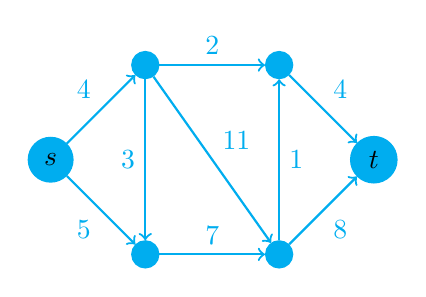
\begin{tikzpicture}[node distance={17mm}, thick, main/.style = {draw, circle, fill}]
		\node[main] (1) [color=cyan] {\textcolor{black}{$s$}};
		\node[main] (2) [above right of=1] [color=cyan] {};
		\node[main] (3) [below right of=1] [color=cyan] {};
		\node[main] (4) [right of=2] [color=cyan] {};
		\node[main] (5) [right of=3] [color=cyan] {};
		\node[main] (6) [below right of=4] [color=cyan] {\textcolor{black}{$t$}};
		\draw[->] (1) -- (2) [color=cyan] node[midway, above left] {4};
		\draw[->] (1) -- (3) [color=cyan] node[midway, below left] {5};
		\draw[->] (2) -- (3) [color=cyan] node[midway, left] {3};
		\draw[->] (3) -- (5) [color=cyan] node[midway, above] {7};
		\draw[->] (2) -- (5) [color=cyan] node[midway, above right] {11};
		\draw[->] (2) -- (4) [color=cyan] node[midway, above] {2};
		\draw[->] (5) -- (4) [color=cyan] node[midway, right] {1};
		\draw[->] (4) -- (6) [color=cyan] node[midway, above right] {4};
		\draw[->] (5) -- (6) [color=cyan] node[midway, below right] {8};
	\end{tikzpicture}
\end{document}